\documentclass[12pt]{article}

\usepackage[pdftex]{graphicx}
\usepackage{subcaption}
\usepackage{float}
\usepackage{url}
\usepackage[utf8]{inputenc}
\usepackage{geometry}
\usepackage{setspace}
\usepackage{amsmath}
\usepackage{txfonts}
\usepackage{hyperref}
\hypersetup{
	colorlinks=true,
	linkcolor=blue,
	filecolor=magenta,      
	urlcolor=cyan,
}

% From amsmath, prepend equation numbers with section number
%\numberwithin{equation}{section}

% graphicx: Where should graphics be found?
\graphicspath{ {figures/} }

% Setup margins and paper size
\geometry{
  letterpaper,
  total={170mm,257mm},
  left=20mm,
  top=20mm,
  bottom=25mm
}

\setcounter{MaxMatrixCols}{20}

\makeatletter % changes the catcode of @ to 11
\renewcommand*\env@matrix[1][*\c@MaxMatrixCols c]{%
  \hskip -\arraycolsep
  \let\@ifnextchar\new@ifnextchar
  \array{#1}}
\makeatother % changes the catcode of @ back to 12

% -----------------------------------------------------------------------------

\begin{document}

% Article Title
\title{\LARGE The Desktop Quad \\ \large with an LQR setpoint controller }
\author{Parker Lusk}
\date{\today}
\maketitle

\begin{abstract}
	This report describes the progress of the Desktop Quad achieving fully autonomous flight.
\end{abstract}

\doublespacing
% -----------------------------------------------------------------------------
\section{Introduction}
The Desktop Quad (see Figure~\ref{fig:sim_pic}) is an effort to allow an inexpensive quadrotor to be used as a case study in controls, vision processing, and autopilot design scenarios. It features an 8cm x 8cm quadrotor with an upward-facing camera for localization. The (really) micro air vehicle (MAV) is tethered using flexible silicone wire for communications and power, allowing indefinite flight. This project aims to close the attitude loop by adding a linear-quadratic regulator (LQR) setpoint controller.

\begin{figure}[H]
	\centering
	\minipage{0.49\textwidth}
	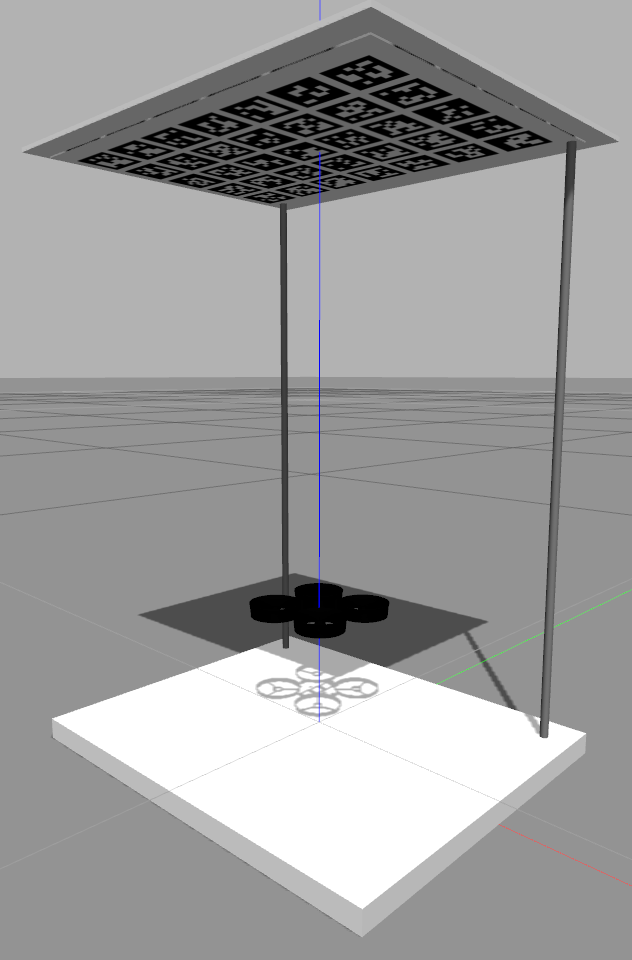
\includegraphics[scale=0.25]{sim_pic}
	\endminipage\hfill
	\minipage{0.49\textwidth}
	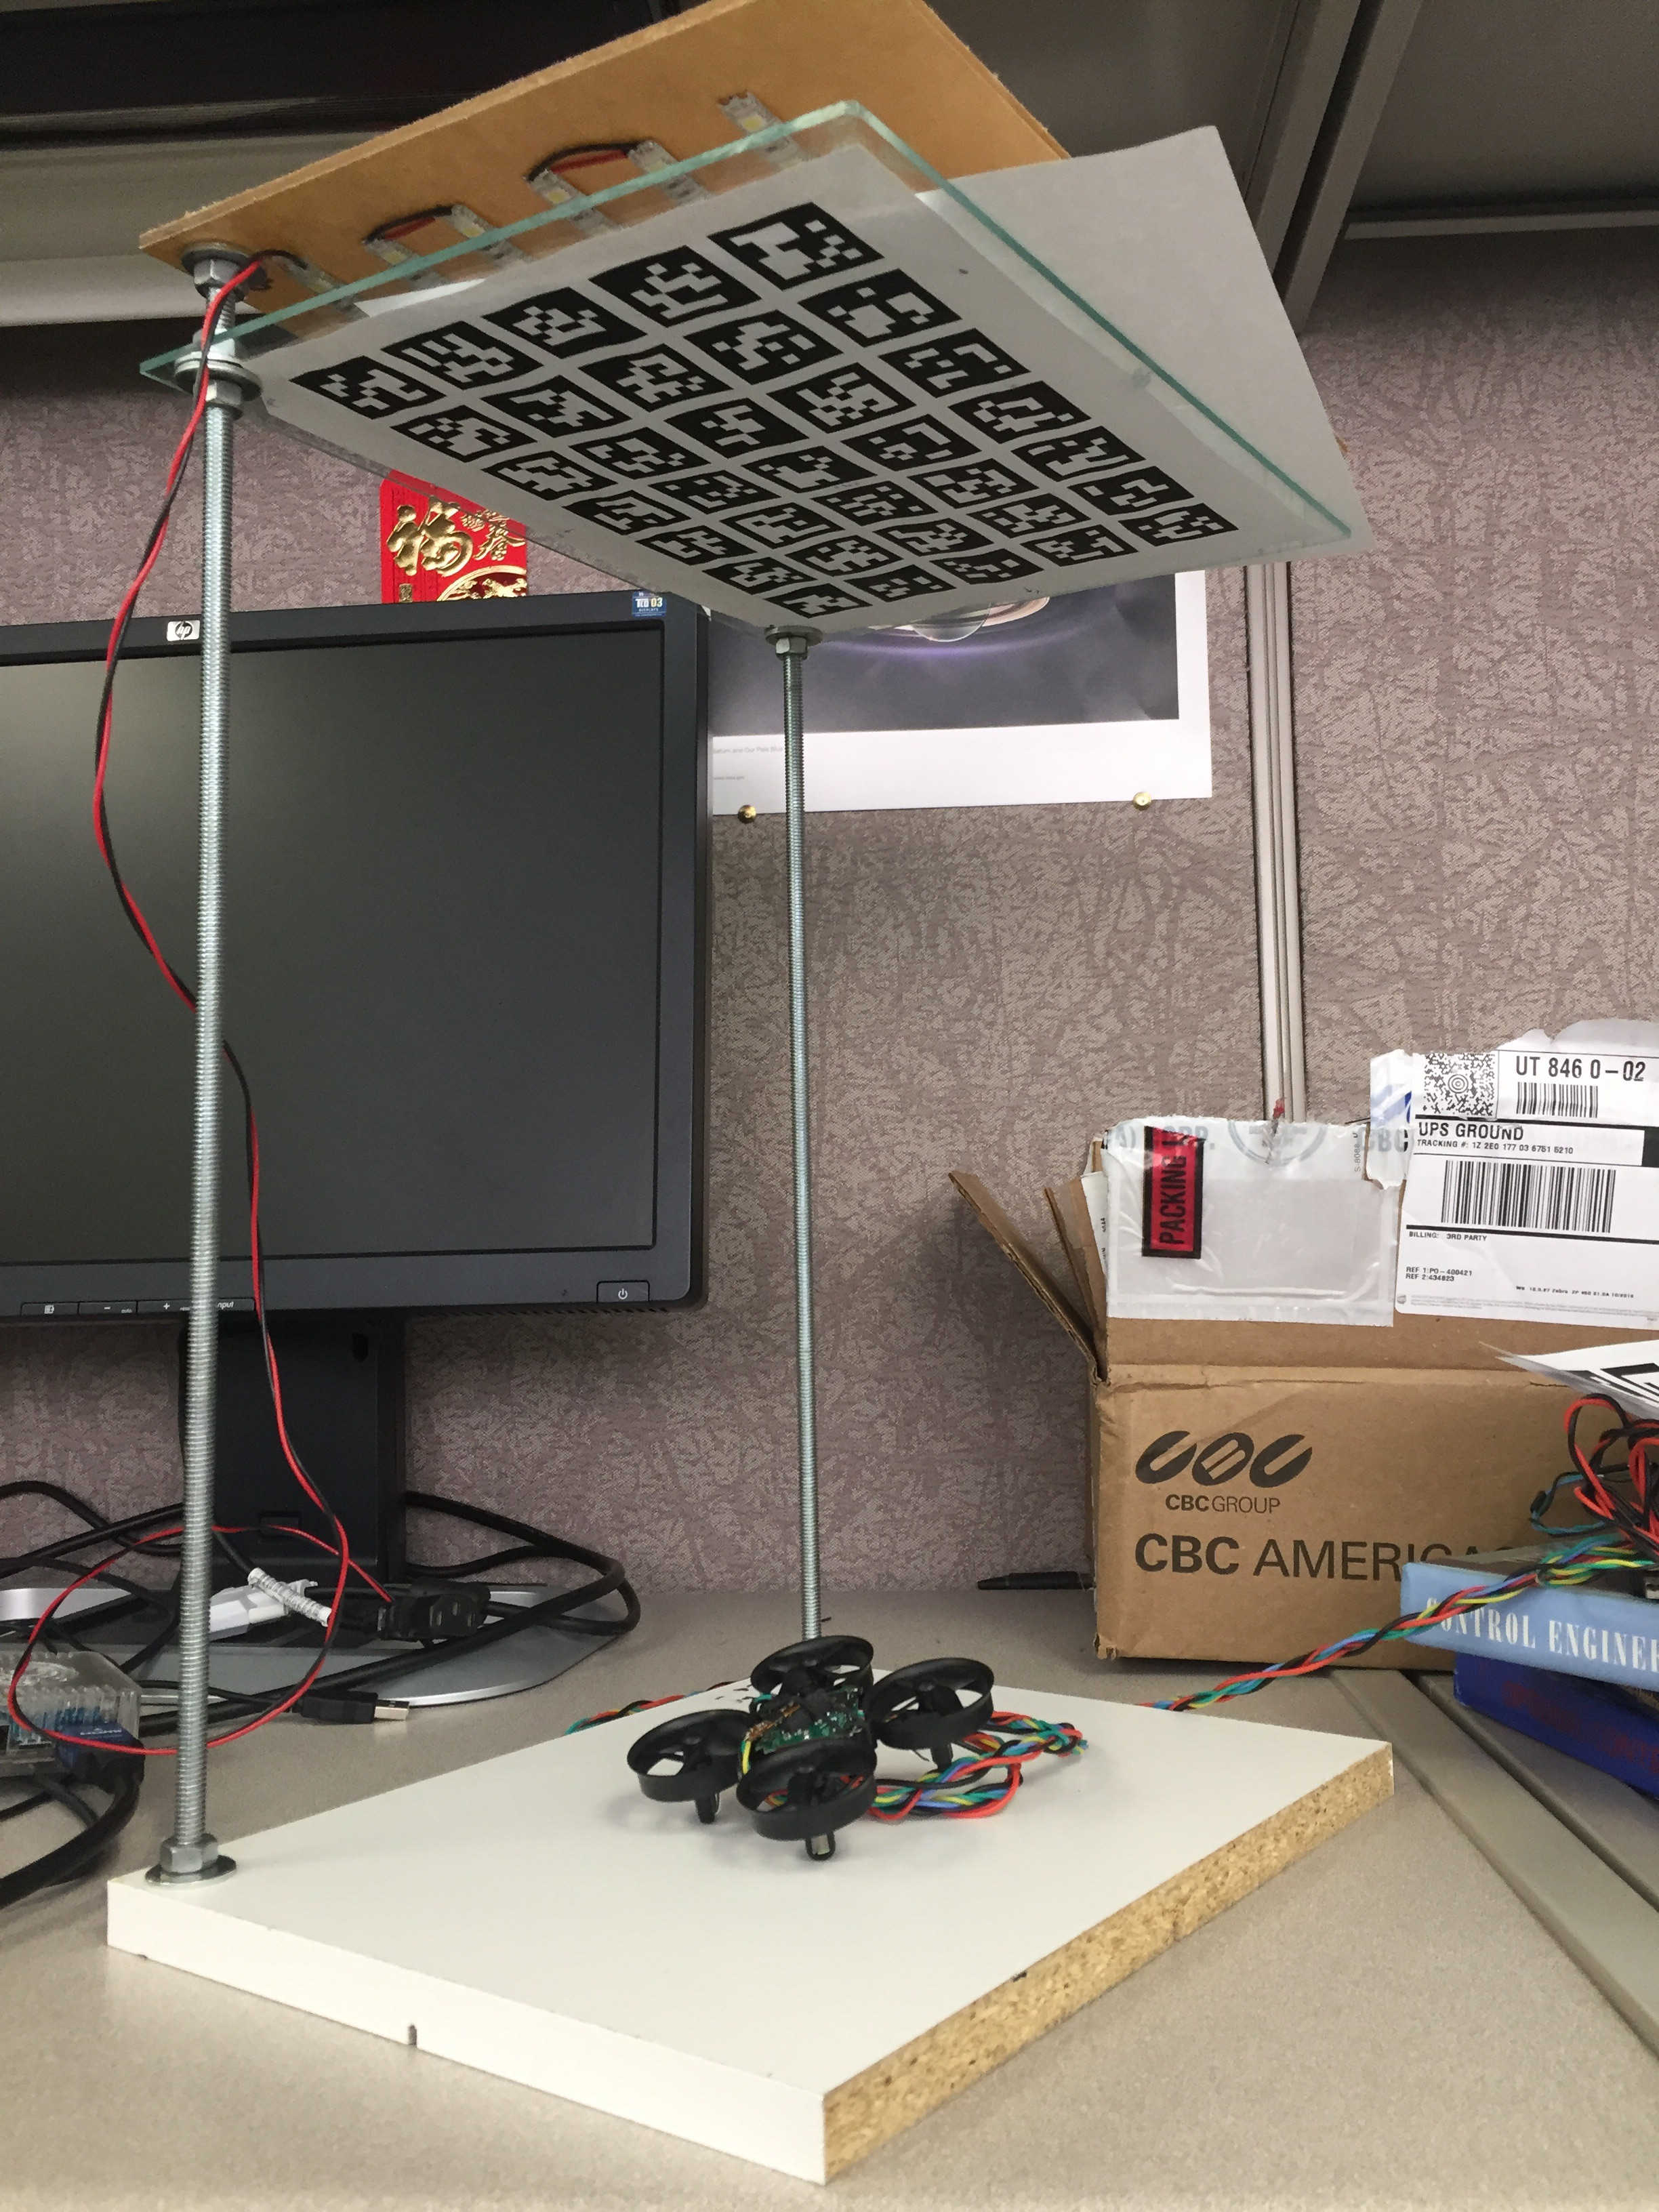
\includegraphics[scale=0.07]{platform}
	\endminipage\hfill
	\caption{The Desktop Quad simulated in Gazebo/ROS, next to the hardware platform.}
	\label{fig:sim_pic}
\end{figure}

% -----------------------------------------------------------------------------
\section{System Modeling}
We begin by modeling the Desktop Quad multirotor and deriving the equations of motion. The 12 state variables that will be used to describe the equations of motions are

\begin{equation*}
x =
\begin{bmatrix}
p_n & p_e & p_d & u & v & w & \phi & \theta & \psi & p & q & r
\end{bmatrix}
^T
\end{equation*}

\noindent where $p_n$, $p_e$, and $p_d$ are inertial north, east, down coordinates; $u$, $v$, $w$ are body frame velocities; $\phi$, $\theta$, $\psi$ are Euler angles; and $p$, $q$, $r$ are body frame angular rates. The two relevant coordinate frames for system modeling are shown in Figure~\ref{fig:multirotor}.

\begin{figure}[H]
	\centering
	\begin{subfigure}{0.45\textwidth}
		\centering
		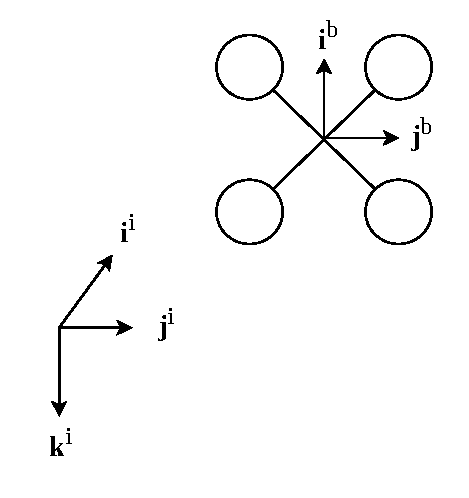
\includegraphics[width=\textwidth]{multirotor}
		\caption{Relevant coordinate frames for modeling}
		\label{fig:multirotor}
	\end{subfigure}
	\begin{subfigure}{0.50\textwidth}
		\centering
		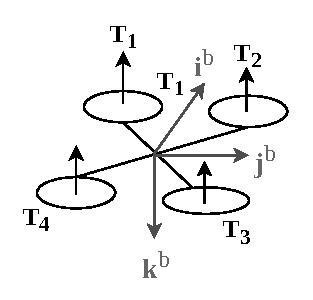
\includegraphics[width=\textwidth]{multirotor_forces}
		\caption{Forces modeled on the quadrotor}
		\label{fig:multirotor_forces}
	\end{subfigure}
	
	\caption{Quadrotor modeling diagrams.}
\end{figure}

\subsection{Kinematics and Dynamics}
In order to analyze, simulate, and control the Desktop Quad, a 6DOF dynamic model must be derived. This is done using kinematics and dynamics. The goal is to find the evolution equations for each of the quantities we care about, as found in the state vector above \cite{UAVBook}.

\singlespacing
\begin{equation}
\begin{bmatrix}
\ddot{p_n} \\
\ddot{p_e} \\
\ddot{p_d} \\
\end{bmatrix}
=
R_b^i(\phi, \theta, \psi)
\begin{bmatrix}
0  \\
0  \\
-T \\
\end{bmatrix}
\frac{1}{m} +
\begin{bmatrix}
0 \\
0 \\
g \\
\end{bmatrix}
\end{equation}
\doublespacing

\singlespacing
\begin{equation}
\begin{bmatrix}
\dot{\phi} \\
\dot{\theta} \\
\dot{\psi} \\
\end{bmatrix}
=
\begin{bmatrix}
1 & s_{\psi}t_{\theta} & c_{\phi}t_{\theta} \\
0 & c_{\phi}           & -s_{\phi}          \\
0 & \frac{s_{\phi}}{c_{\theta}} & \frac{c_{\phi}}{c_{\theta}} \\
\end{bmatrix}
\begin{bmatrix}
p \\
q \\
r \\
\end{bmatrix}
\end{equation}
\doublespacing

\singlespacing
\begin{equation}
\begin{bmatrix}
\dot{p} \\
\dot{q} \\
\dot{r} \\
\end{bmatrix}
=
\begin{bmatrix}
\Gamma_1pq - \Gamma_2qr \\
\Gamma_5pr - \Gamma_6(p^2-r^2) \\
\Gamma_7pq - \Gamma_1qr \\
\end{bmatrix}
+
\begin{bmatrix}
\Gamma_3l + \Gamma_4n \\
\frac{1}{J_y}m \\
\Gamma_4l + \Gamma_8n \\
\end{bmatrix}
\end{equation}
\doublespacing

\noindent where $T = T_1 + T_2 + T_3 + T_4$, $m$ is the mass of the multirotor, and the trigonometric functions are shortened as shown.

%\subsection{Forces and Moments}

% -----------------------------------------------------------------------------
\section{Control Architecture}

\begin{figure}[H]
	\centering
	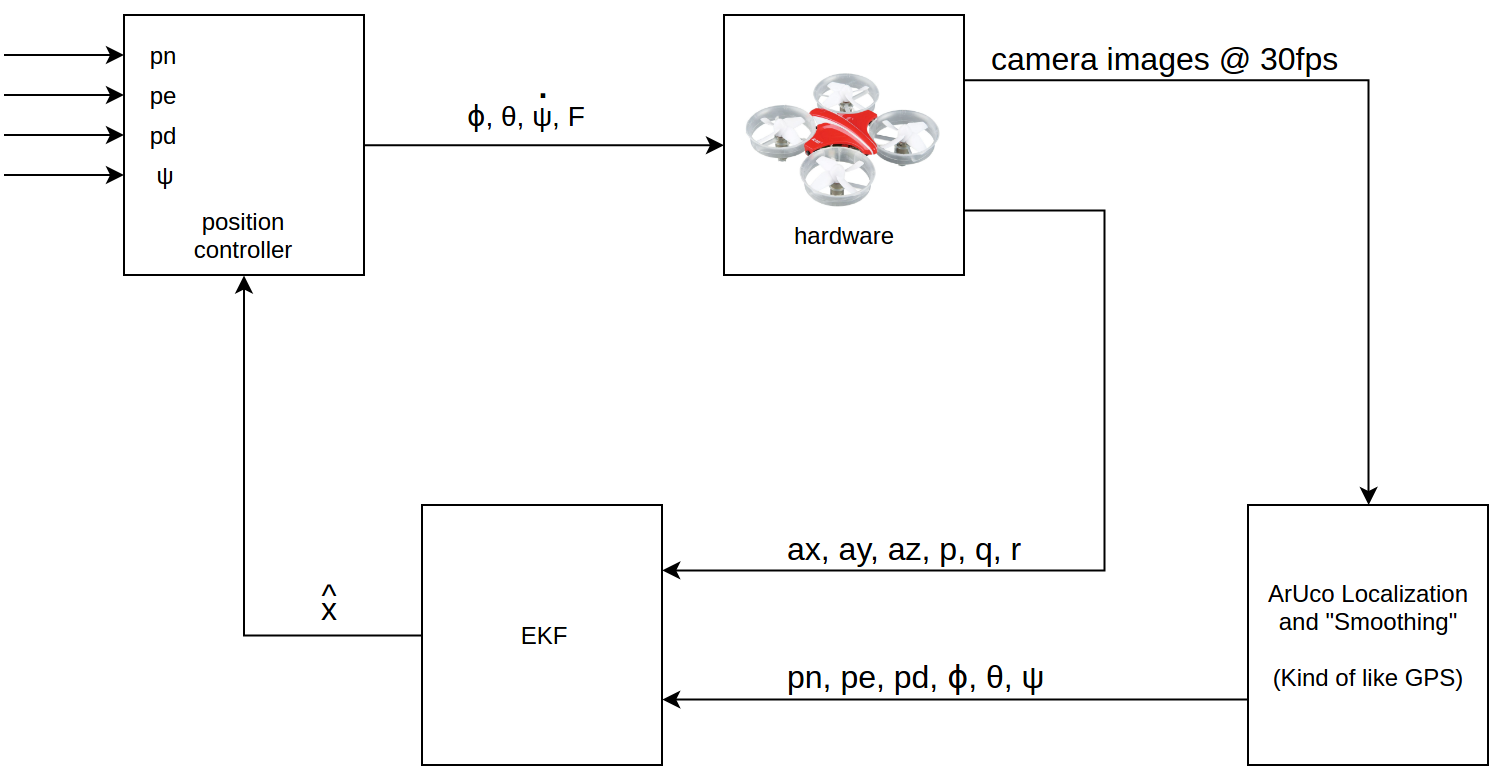
\includegraphics[scale=0.23]{desktopquad_control_arch}
	\caption{Control architecture of the Desktop Quad system.}
	\label{fig:architecture}
\end{figure}

The Desktop Quad uses the ROSflight \cite{rosflight} stack for autonomous flight and thus has an on-board autopilot for attitude control. This simplifies the control problem and eliminates the need to control the moments $l$, $m$, and $n$. The LQR controller developed here will close the attitude loop using a position setpoint controller as shown in Figure~\ref{fig:architecture}. The simplified outer-loop state vector is defined as

\singlespacing
\begin{equation*}
x =
\begin{bmatrix}
p_n & p_e & p_d & \dot{p_n} & \dot{p_e} & \dot{p_d} & \psi
\end{bmatrix}
^T
\end{equation*}
\doublespacing

\noindent with input to the ROSflight autopilot

\singlespacing
\begin{equation*}
\nu =
\begin{bmatrix}
T & \phi & \theta & r
\end{bmatrix}^T.
\end{equation*}
\doublespacing

Because of how we have defined our state, we will need to create a nonlinear map between the control $u$ produced by our controller and the input $\nu$ to the autopilot. We can use the kinematic and dynamic relationships to define the map

\begin{equation}
\boldsymbol{u} = 
\begin{bmatrix}
u_{p_{3x1}} \\
u_{{\psi}_{1x1}}
\end{bmatrix},
\end{equation}

\noindent where

\begin{equation}
u_p =
R_b^i(\phi, \theta, \psi)
\begin{bmatrix}
0  \\
0  \\
-T \\
\end{bmatrix}
\frac{1}{m}
\end{equation}

\noindent and

\begin{equation}
u_{\psi} =
q\frac{sin\phi}{cos\theta} + r\frac{cos\phi}{cos\theta}.
\end{equation}

\noindent Inverting these relationships will give us a mapping for how $u$ affects $\nu$, which can be feed into autopilot. The state-space system can be represented as

\begin{equation}
\dot{x} = Ax + Bu + bg
\end{equation}

\noindent with


\begin{equation}
A =
\begin{bmatrix}
0_{3x3} & I_{3x3} & 0_{3x1} \\
0_{3x3} & 0_{3x3} & 0_{3x1} \\
0_{1x3} & 0_{1x3} & 0_{1x1} \\
\end{bmatrix}
, \quad
B =
\begin{bmatrix}
0_{3x3} & 0_{3x1} \\
I_{3x3} & 0_{3x1} \\
0_{1x3} & 1 \\
\end{bmatrix}
, \quad
b = [0 \enspace 0 \enspace 0 \enspace 0 \enspace 0 \enspace 1 \enspace 0]^T.
\end{equation}

\begin{figure}[H]
	\centering
	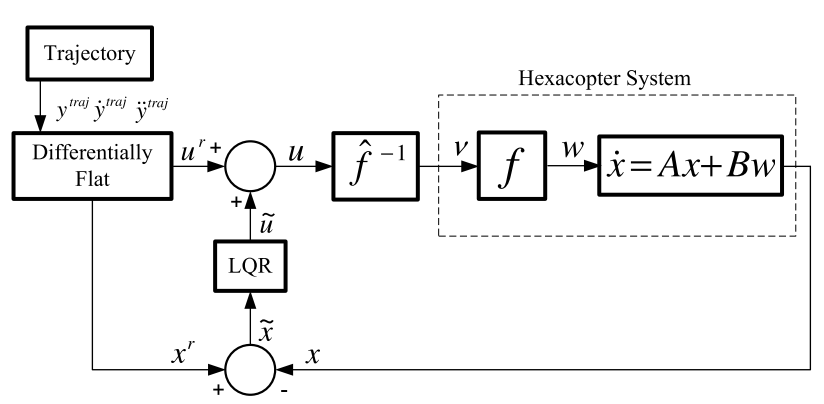
\includegraphics[scale=0.50]{diff_flat}
	\caption{Differentially flat / LQR controller, shamefully stolen from \cite{Ferrin2011}.}
	\label{fig:diff_flat_arch}
\end{figure}

% -----------------------------------------------------------------------------
\section{Differential Flatness}

A differentially flat system is one in which the state and control inputs can be expressed as functions of the output and its time derivatives. Formulating the problem this way let's us use these properties to create a 2nd order trajectory that the multirotor will follow. If our models were perfect, the differentialy flat block of Figure~\ref{fig:diff_flat_arch} would only need to output a control $u$ that then would go into the model. Because we should never take our models (or ourselves) too seriously, we add LQR to regulate our error state to 0.

% -----------------------------------------------------------------------------
%\section{Linear-Quadratic Regulator}

% -----------------------------------------------------------------------------
\section{Simulation Environment}

The LQR setpoint controller was first designed in MATLAB / Simulink based on the MAGICC lab Mikrocopter Hexacopter simulation. Along with the setpoint controller, a differential flatness \cite{Ferrin2011} trajectory generator was implemented to compare and contrast against. Figure~\ref{fig:matlab_hex_sim} shows the Simulink diagram and how the differential flatness trajectory or the setpoint can be selected during the simulation.

\begin{figure}[H]
	\centering
	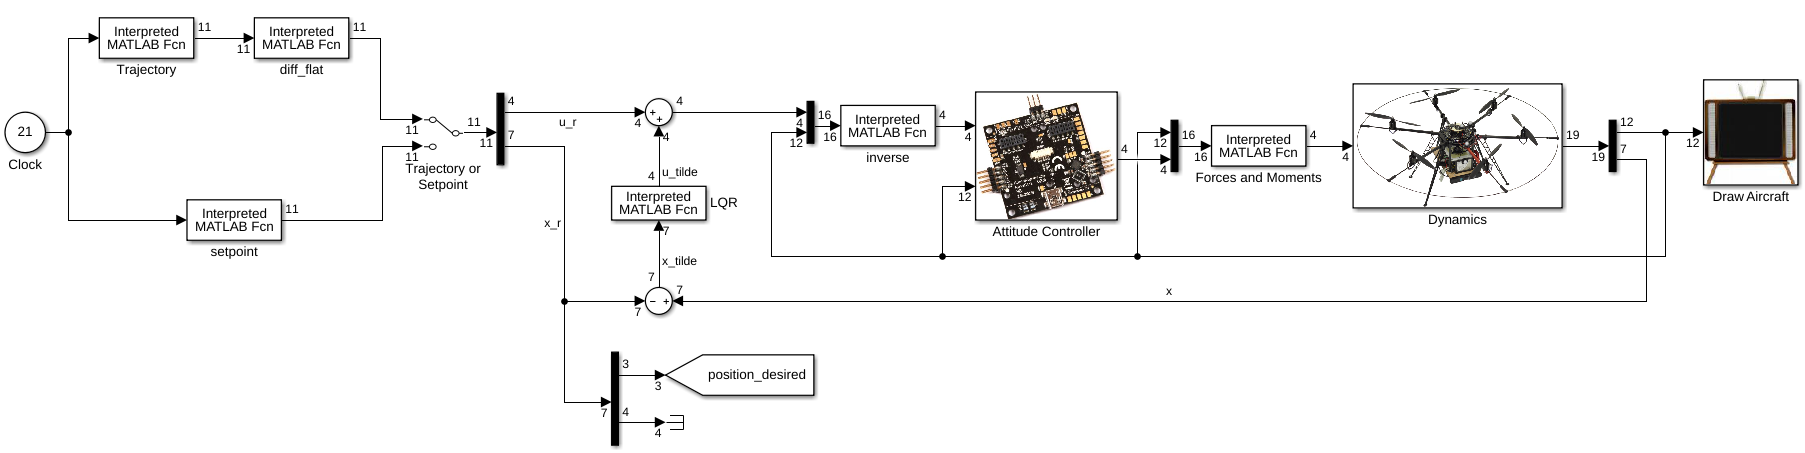
\includegraphics[scale=0.28]{hex_sim}
	\caption{The LQR setpoint controller design simulated in MATLAB/Simulink.}
	\label{fig:matlab_hex_sim}
\end{figure}

After developing and tuning the control algorithm in MATLAB using the \texttt{lqr} command, the design and gains were then ported to C++ for ROS/Gazebo. Using ROS allows the same implementation to be used in the Desktop Quad simulator and directly in hardware (see Figure~\ref{fig:sim_pic}).

% -----------------------------------------------------------------------------
\section{Results}

Results of using the setpoint and differential flatness controllers can be found in Figures~\ref{fig:matlab_setpoint_results}~and~\ref{fig:matlab_diff_flat_results} respectively. Video results of the MATLAB and ROS simulations can be shown \href{https://youtu.be/hX0MF_FHCtE}{here} and \href{https://youtu.be/GLhXQmhUx8w}{here}.

\begin{figure}[H]
	\centering
	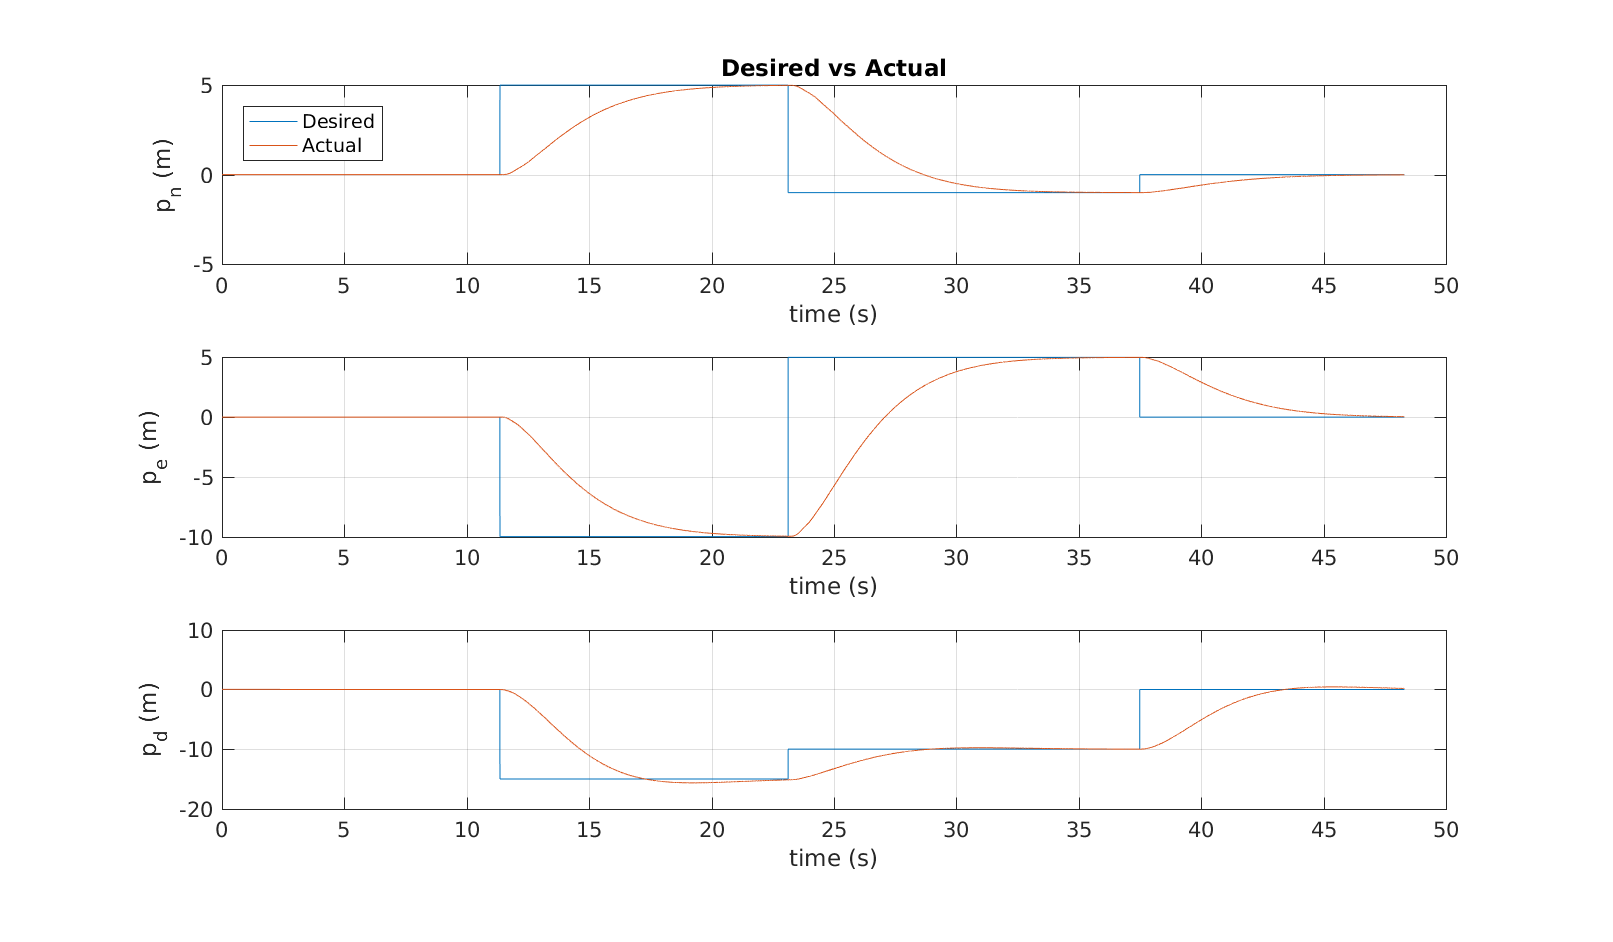
\includegraphics[scale=0.55]{hex_sim_desired_vs_actual}
	\caption{Error of the commanded and actual positions using the setpoint controller.}
	\label{fig:matlab_setpoint_results}
\end{figure}

\begin{figure}[H]
	\centering
	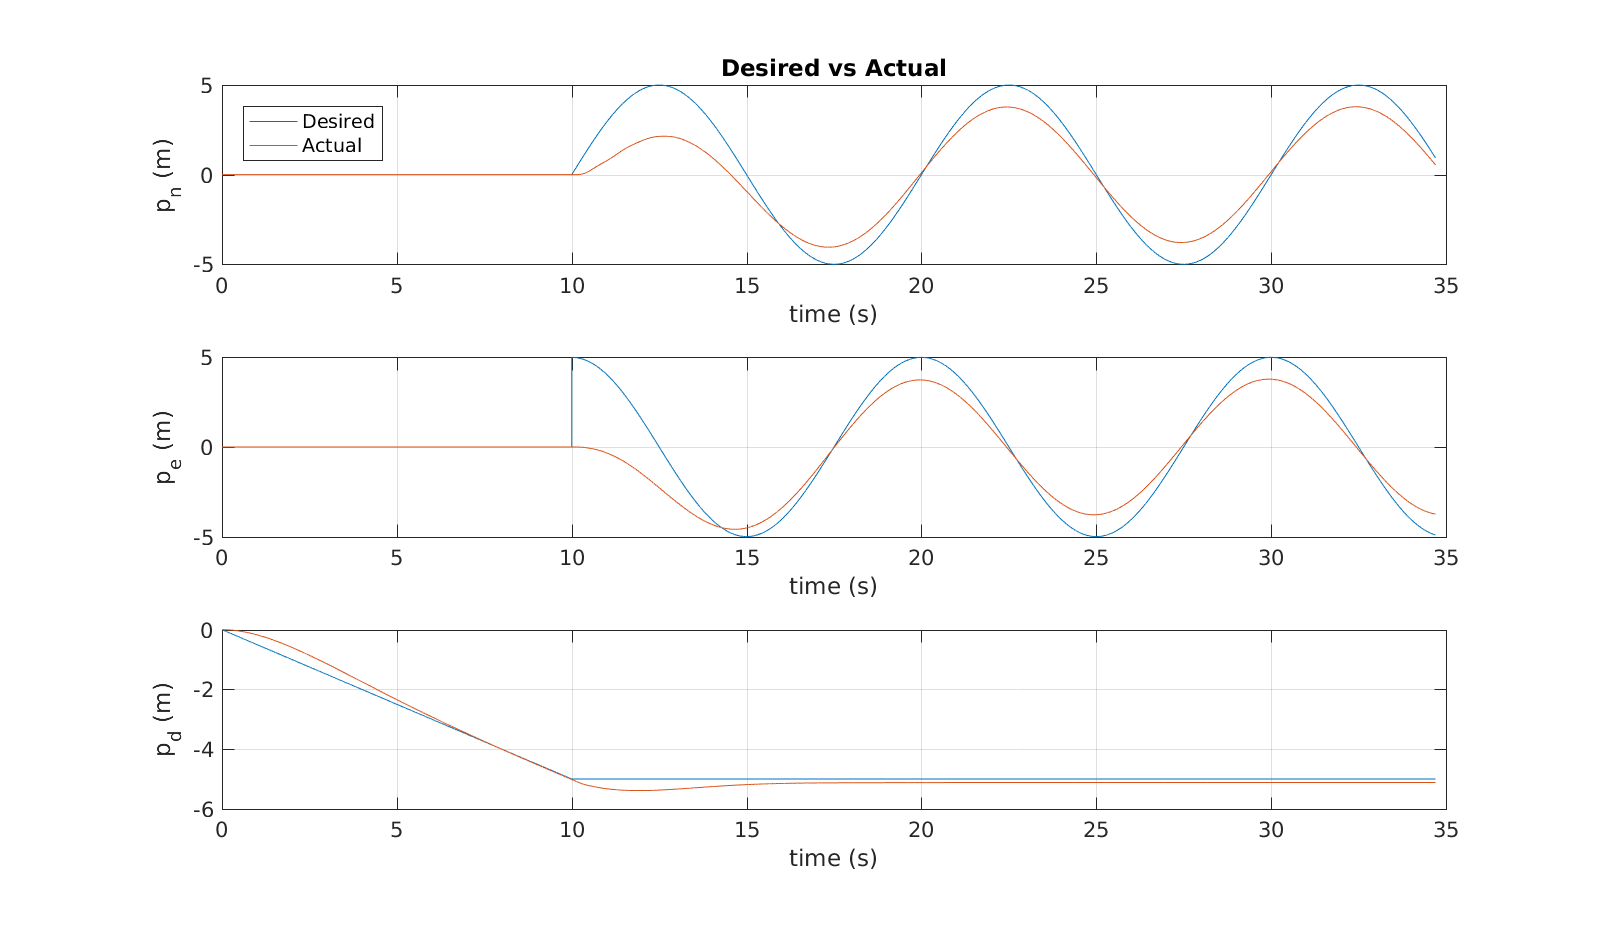
\includegraphics[scale=0.55]{hex_sim_desired_vs_actual_diff_flat}
	\caption{Error of the commanded and actual positions using the differential flatness trajectory generator.}
	\label{fig:matlab_diff_flat_results}
\end{figure}

% -----------------------------------------------------------------------------
\section{Conclusion}

Using the differential flatness properties of the quadrotor system allows intuitive control of the outer position loop. As a result of using LQR to regulate the error state $\tilde{x}$ to $0$, the controlled motion is very smooth and stable.

It was good for me to implement the differentially flat LQR controller in MATLAB and C++. I was able to further understand the importance and use of the feedforward gain  $N$ and the state gain $F$.

I noticed in the Gazebo simulation that I had more steady-state error than in the MATLAB simulation. I would like to add an integrator to the position states to further improve my control accuracy.

\begin{thebibliography}{9}
\singlespace

\bibitem{UAVBook} R. W. Beard and T. W. McLain, “Small unmanned aircraft,” 2011.

\bibitem{Beard2016} R. W. Beard and T. W. Mclain, “Introduction to Feedback Control using Design Studies,” 2016.

\bibitem{Ferrin2011} J. Ferrin, R. Leishman, R. Beard, and T. McLain, “Differential flatness based control of a rotorcraft for aggressive maneuvers,” IEEE Int. Conf. Intell. Robot. Syst., pp. 2688–2693, 2011.

\bibitem{rosflight} J. Jackson, G. Ellingson, and T. McLain, “ROSflight: A lightweight, inexpensive MAV research and development tool,” 2016 Int. Conf. Unmanned Aircr. Syst. ICUAS 2016, pp. 758–762, 2016.

\end{thebibliography}

\end{document}